%Tex root = Linguaggi.tex

\chapter{Identificatori}
\begin{mydef}{identificatore}
    Un \textbf{identificatore} è una sequenza alfa-numerica di caratteri usate per denotare e riferire oggetti di varia natura.
    \[
        \begin{aligned}
            &\texttt{const pi = 3,14} &\texttt{//denota un valore}\\
            &\texttt{int x} &\texttt{//denota una variabile}\\
            &\texttt{void f()\{...\}} & \texttt{//definisce una funzione (procedura)}
        \end{aligned}
    \]
\end{mydef}

Bisogna ricordare che:
\[
    \mathbf{identificatore} \neq \mathbf{oggetto \ denotato}
\]

Infatti, è possibile avere più identificatori che si riferiscono allo stesso oggetto (aliasiang).

%foto??

E' possibile, anche che più oggetti denotati dallo stesso identificatori (polimorfismo).

\medskip
I linguaggi di programmazione possono porre delle regole (limiti) a quello che piò essere usato come identificatore:
\begin{itemize}[label=$\triangleright$, itemsep=\smallskipamount]
    \item \textbf{sono oppure no case sensitive?}
    \[
        \text{in } \texttt{C pippo, Pippo, PIPPO } \text{sono identificatori diversi}
    \]
    \item \textbf{essitono parole riservate?}: parole riservate perchè già associate a specifici significati
    \item \textbf{esistono restrizioni sulla lunghezza?}
    \[
        \begin{aligned}
            &\texttt{FORTRAN}: \text{massimo } 31 \text{ caratteri}\\
            &\texttt{C}: \text{caratteri illimitati}
        \end{aligned}
    \]
    \item \textbf{ci sono cattteri speciali da utilizzare?}
    \[
        \text{in } \texttt{PHP } \text{devono iniziare con il simbolo } \$
    \]
\end{itemize}

\section{Legame}
Il concetto di \textbf{binding} (legame) viene ereditato dalla matematica.

\begin{figure}[htbp]
     \centering
     % Prima immagine
     \begin{subfigure}[b]{0.3\textwidth}
         \centering
         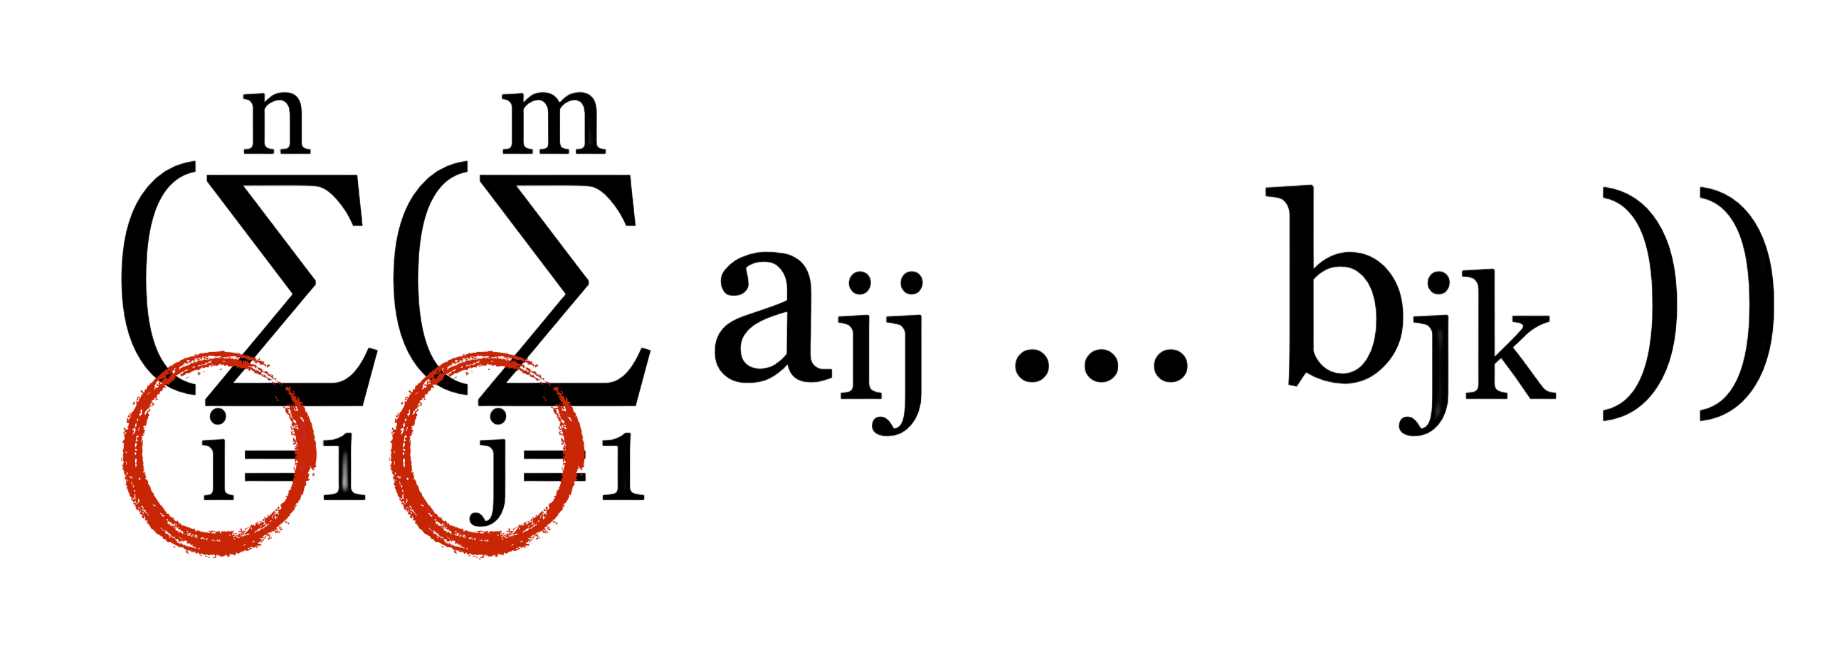
\includegraphics[width=\textwidth]{images/occorrenza-legame.png}
         \caption{occorrenza di legame}
     \end{subfigure}
     \hfill % Spazio flessibile tra le immagini
     % Seconda immagine
     \begin{subfigure}[b]{0.3\textwidth}
         \centering
         
\includegraphics[width=\textwidth]{images/occorrenza-applicazione.png}
         \caption{occorrenza di applicazione}
     \end{subfigure}
     \hfill
     % Terza immagine
     \begin{subfigure}[b]{0.3\textwidth}
         \centering
         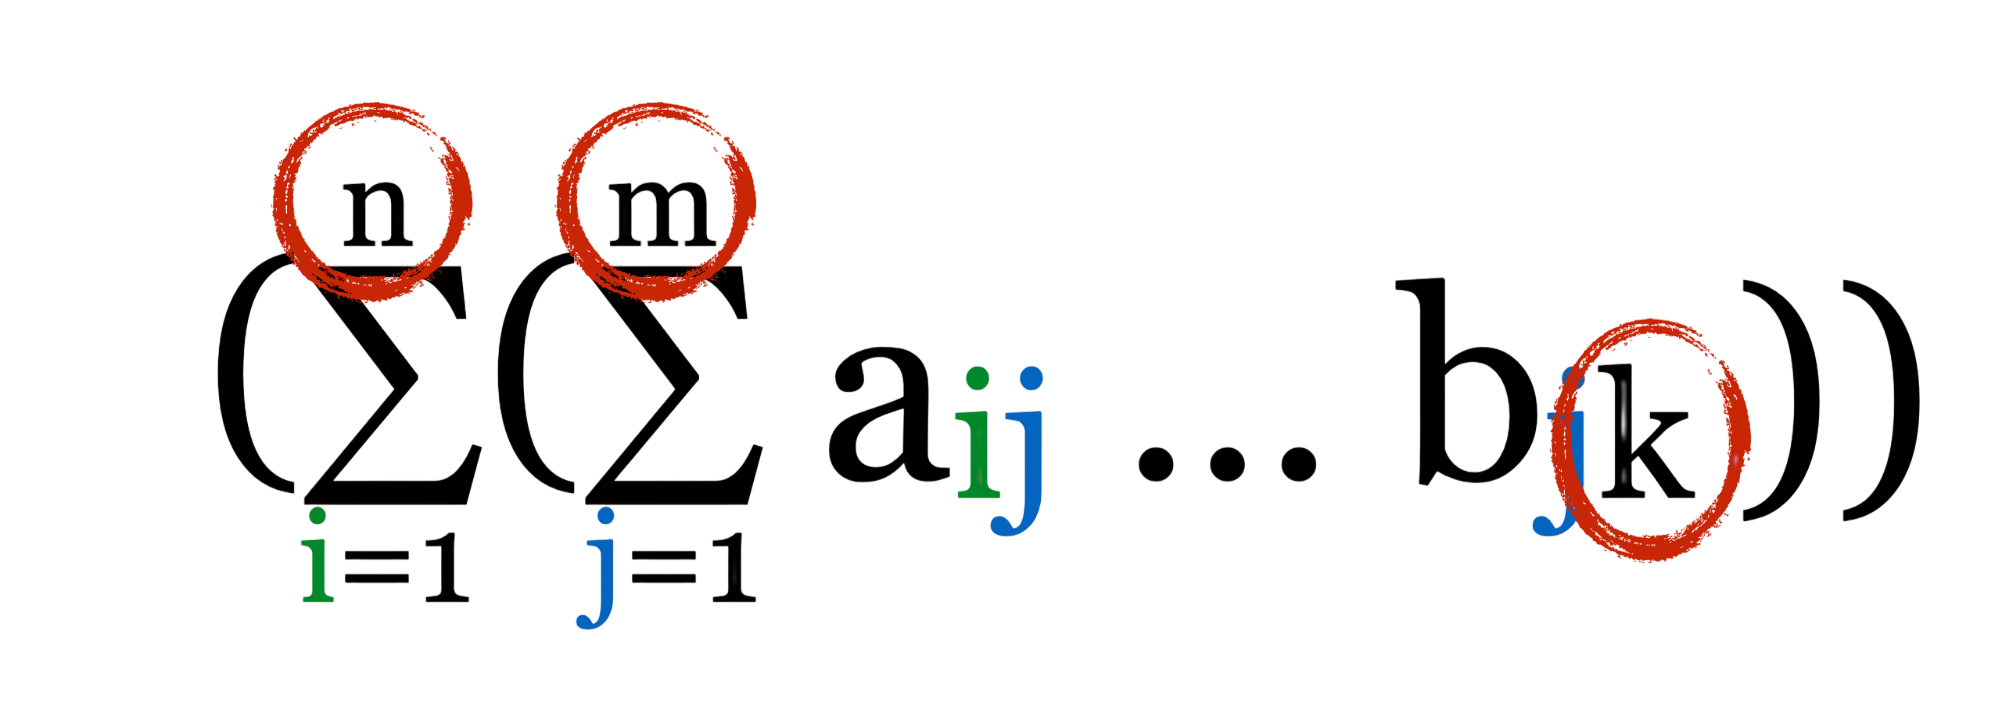
\includegraphics[width=\textwidth]{images/occorrenza-libera.png}
         \caption{occorrenza libera}
     \end{subfigure}
\end{figure}

\begin{mydef}{occorrenza di legame}
    Con l'\textbf{occorrenza di legame} viene creato il legame tra nome e il suo significato.
\end{mydef}

\begin{mydef}{occorrenza di applicazione}
    Con l'\textbf{occorrenza di applicazione} viene usato il nome per accedere al suo significato.
\end{mydef}

\begin{mydef}{occorrenza libera}
    Con l'\textbf{occorrenza libera} viene usato un nome a cui non è stato associato nessun significato.
\end{mydef}

Dal punto di vista del costrutto le occorrenze libere e quelle applicate sono identiche, la differenza consiste nell'essere nel raggio di azione (scope) di una occorrenza di definizione.

\begin{mydef}{scope di un binding}
    Lo \textbf{scope} definisce lo spazio in cui si può usare un nome per rappresentare il significato associato a un binding.
\end{mydef}

\begin{figure}[H]
    \centering
    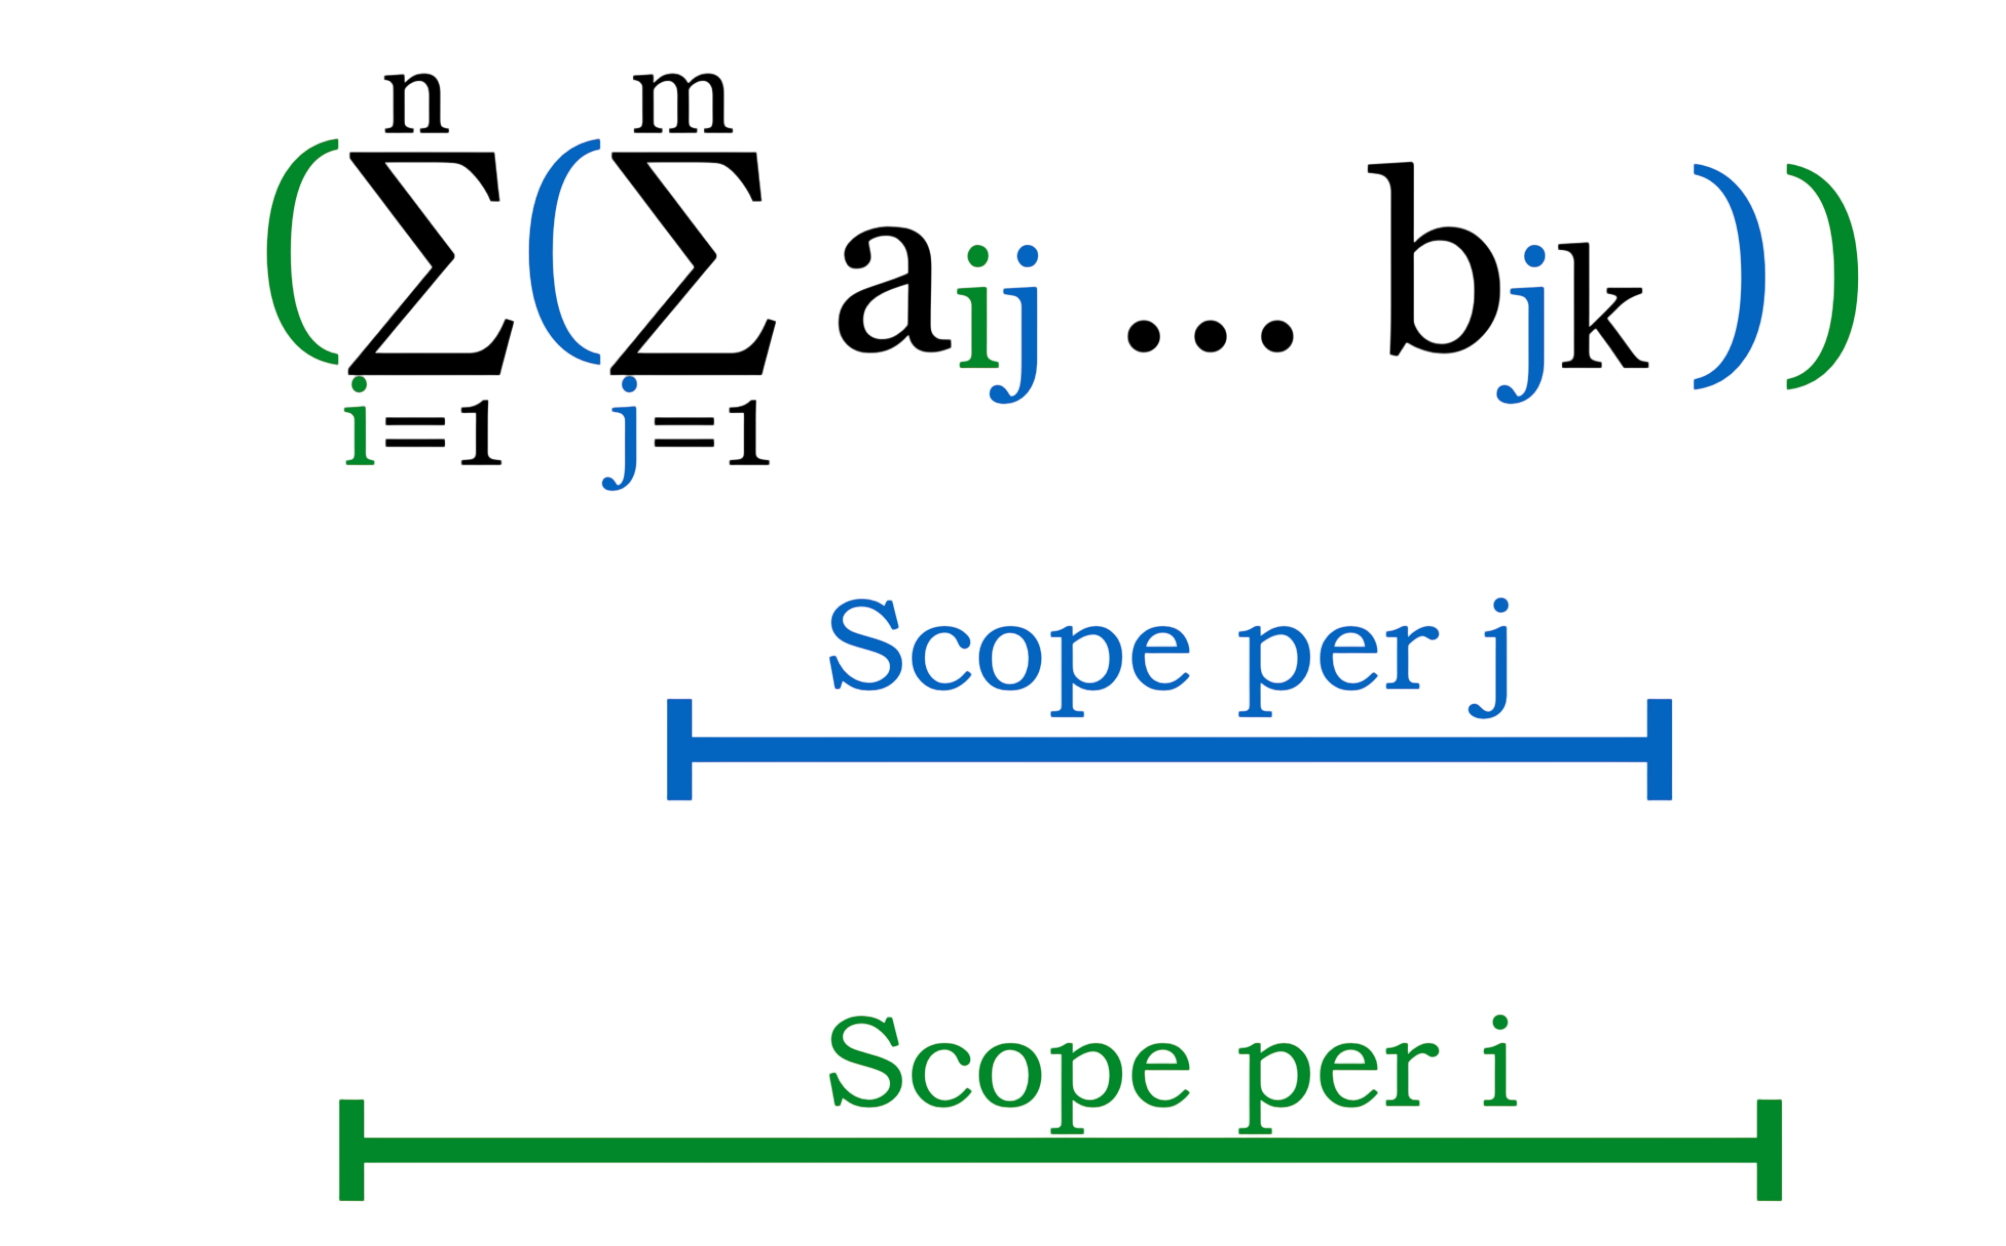
\includegraphics[width=0.4\textwidth]{images/scope-binding.png}
    \caption{scope di un binding}
\end{figure}

\smallskip
Nei linguaggi di programmazione i concetti di binding e scope prendono una connotazione propria:
\begin{itemize}[label=$\circ$, itemsep=\smallskipamount]
    \item \textbf{definizione} (occorrenza di legame): un identificatore è in posizione di definizione quando si definisce il suo significato (si crea il legame)
    \item \textbf{uso} (occorrenza di applicazione): un identificatore è in fase d'uso quando si riferisce al significato associato da una specifica definizione
    \item \textbf{libera} (occorrenza libera): un indentificatore è in posizione libera se il suo uso è nel raggio di azione di nessuna definizione
\end{itemize}

\subsection{Tipi di binding}
Distingue i binding rispetto alla durata del legame e sulla dinamicità del legame.
\begin{itemize}[itemsep=\smallskipamount]
    \item[$\diamond$] $\left. 
    \begin{array}{l} 
        \mathbf{nome} \leftrightarrow \mathbf{valore}\\ 
        \mathbf{nome} \leftrightarrow \mathbf{locazione} 
    \end{array} \right\} $ legami in cui l'oggetto denotato non cambia (binding statico)
    \item[$\diamond$] $\mathbf{locazione} \leftrightarrow \mathbf{valore} \rightarrow$ legame in cui l'ogetto denotato può cambiare (binding dinamico)
\end{itemize}

\subsection{Tempo di binding}
Distingue i binding rispetto al momento in cui il binding viene creato.
\begin{itemize}[label=$\diamond$, itemsep=\smallskipamount]
    \item \textbf{tempo compilazione} (eraly binding): \texttt{FORTRAN}, \texttt{C}, \texttt{COBOL}
    \begin{itemize}[itemsep=\smallskipamount]
        \item esecuzione veloce
        \item non flessibile
        \item uso dello stack (allocazione statica)
    \end{itemize}
    \item \textbf{tempo di esecuzione} (late binding): \texttt{SNOBOL4}, \texttt{LISP}, \texttt{APL}
    \begin{itemize}[itemsep=\smallskipamount]
        \item esecuzione lenta
        \item flessibile
        \item uso dello heap
    \end{itemize}
\end{itemize}

\section{Ambiente}
I legami vengono inseriti nell'ambiente (insieme di binding).\\[0.2ex]
Le \textbf{dichiarazioni} sono il meccanismo (implicito o esplcito) che permette di modificare gli ambienti.

\smallskip
Nelle espressioni abbiamo solo identificatori lberi, ma se vogliamo dare loro significati dobbiamo rendere tali occorrenze applicate inserendole nello scope di binding.

\smallskip
Ci sono due tipi di termini:
\begin{itemize}[label=$\triangleright$, itemsep=\smallskipamount]
    \item \textbf{termine ground}: termine che non contiene identificatore
    \item \textbf{termine chiuso}: termine in cui non ci sono identificatori liberi
\end{itemize}

Entrambi i tipi di termini hanno significato senza dover riccorrere a un contesto esterno (ambiente).

\section{Sintassi}
Riprendiamo la seguente notazione:
\begin{itemize}[label=$\diamond$, itemsep=\smallskipamount]
    \item $\mathcal{E}$: insieme delle espressioni
    \item $\mathcal{D} \mathrm{Val} = \mathcal{N} \cup \mathcal{B}$: insiem dei valori numerici e booleani (valori denotabili)
\end{itemize}

Definiamo formalmente l'ambiente per le espressioni:
\begin{mydef}{ambiente}
    L'\textbf{ambiente} è un elemento dello spazio delle funzioni:
    \[
        \mathrm{Env} = \bigcup\limits_{\mathrm{V} \ \subseteq{f} \ \mathrm{Id}} \mathrm{Env_V}
    \]

    dove:
    \begin{itemize}[label=$\circ$, itemsep=\smallskipamount]
        \item $\mathrm{Env_V} : \mathrm{V} \rightarrow \mathrm{Val}$
        \item $\cup \{\bot\}$ ha una metavariabile $\rho$
    \end{itemize}
\end{mydef}

A questo punto possiamo completare la sintassi delle espressioni:
\begin{bnfcode}{Sintassi delle espressioni}
    <Exp>
    E -> A | B
    A -> I | n | A op A
    B -> I | true | false | not B | B or B | A = A
\end{bnfcode}

dove:
\begin{itemize}[label=$\triangleright$, itemsep=\smallskipamount]
    \item \texttt{I}: identificatore
\end{itemize}

\subsection{Identificatore libero}
Data un'espressione o una frase scritta in un certo linguaggio, gli identificatori lberi sono quelli che non hanno nessuna dichiarazione che li coinvolge.\\[0.2ex]
Questo significa che la frase in questione è necessariamente parte di una frase più grande dove gli identificatori liberi sono legati e trovano significato.

\begin{mydef}{identificatore libero}
    La funzione:
    \[
        \mathrm{FI} : \mathrm{Exp} \rightarrow \mathrm{Id}
    \]

    che ad ogni espressione associa l'insieme degli identificatori liberi in essa contenuti, è definita da:
    \begin{itemize}[label=$\triangleright$, itemsep=\smallskipamount]
        \item $\mathrm{FI} = \emptyset$
        \item $\mathrm{FI}(\mathrm{id}) = \{\mathrm{id}\}$
        \item $\mathrm{FI}(\mathrm{e_0} \verb| op | \mathrm{e_1}) = \mathrm{FI}(\mathrm{e_0}) \cup \mathrm{FI}(\mathrm{e_1}) = \mathrm{FI}(\mathrm{e_0} \verb| or | \mathrm{e_1}) = \mathrm{FI}(\mathrm{e_0} \verb| = | \mathrm{e_1})$
        \item $\mathrm{FI}(\verb|not | \mathrm{e_0}) = \mathrm{FI}(\mathrm{e})$
    \end{itemize}
\end{mydef}

\esempio{identificatore libero di un'espressione}{
    Consideriamo l'espressione:
    \[
        \mathcal{E} = \mathrm{x + 5y + 3}
    \]

    L'identificatore libero corrisponde a:
    \[
        \begin{aligned}
             &\mathrm{FI}(\mathrm{x + 5y + 3})\\
            = &\mathrm{FI}(\mathrm{x}) \cup \mathrm{FI}(\mathrm{5y}) \cup \mathrm{FI}(\mathrm{3})\\
            = &\{\mathrm{x}\} \cup \mathrm{FI}(\mathrm{5y}) \cup \mathrm{FI}(\mathrm{3})\\
            = &\{\mathrm{x}\} \cup \{\mathrm{y}\} = \{\mathrm{x, y}\} 
        \end{aligned}
    \]
}

Così come possiamo definire gli indentificatori liberi, possiamo definire anche anche quelli definiti $\mathrm{DI}$ (sempre per induzione sulla struttura sintattica delle espressioni).\\[0.2ex]
La definizione è molto semplice in quanto nelle espressioi non abbiamo costruttu che creano legami, occorrenze, ma solo costrutti che utilizzano occorrenze.\\[0.2ex]
Quindi, l'insieme delle occorrenze legate/definite è vuoto ($\mathrm{DI(e)} = \emptyset$).

\section{Semantica}

\subsection{Regole di transizione}
Definiamo la semantica per le espressioni da valuatare in un ambiente $\rho$:
\[
    \rho \vdash \mathrm{e} \rightarrow \mathrm{e}'
\]

Ciò significa che l'espressione $\mathrm{e}$ viene valutata in $\mathrm{e}'$ nell'ambiente $\rho$.\\[0.2ex]
Le regole di transizione per le espressioni con indentificatori diventano:
\begin{itemize}[label=$\triangleright$, itemsep=\smallskipamount]
    \item \textbf{regola 1} (assioma):
    \vario{regola $\mathcal{E}_1$ (assioma)}{
        \[
            \mathcal{E}_1: \rho \vdash m \texttt{ op } n \rightarrow p \quad \Leftrightarrow \quad m \texttt{ op } n = p
        \]
    }
    \item \textbf{regola 2}:
    \vario{regola $\mathcal{E}_2$}{
        \[
           \mathcal{E}_2: \rho \vdash I \rightarrow_e n \quad \Leftrightarrow \quad \rho(I) = n
        \]
    }
    \item \textbf{regola 3}:
    \vario{regola $\mathcal{E}_3$}{
        \[
           \mathcal{E}_3:\;
           \begin{prooftree}
            \hypo{\rho \vdash e \rightarrow_e e'}
            \infer1{\rho \vdash e \texttt{ op } e_0 \rightarrow_e e' \texttt{ op } e_0}
           \end{prooftree}
        \]
    }
    \item \textbf{regola 4}:
    \vario{regola $\mathcal{E}_4$}{
        \[
           \mathcal{E}_4:\;
           \begin{prooftree}
            \hypo{\rho \vdash e \rightarrow_e e'}
            \infer1{\rho \vdash m \texttt{ op } e \rightarrow_e m \texttt{ op } e'}
           \end{prooftree}
        \]
    }
    \item \textbf{regola 5}:
    \vario{regola $\mathcal{E}_5$}{
        \[
           \mathcal{E}_5:\;
           \begin{prooftree}
            \hypo{\rho \vdash e \rightarrow_e e'}
            \infer1{\rho \vdash \texttt{not } e \rightarrow_e \texttt{not } e'}
           \end{prooftree}
        \]
    }
    \item \textbf{regola 6}:
    \vario{regola $\mathcal{E}_6$}{
        \[
           \mathcal{E}_6: \rho \vdash \texttt{not } t \rightarrow t' = \texttt{not } t
        \]
    }
    \item \textbf{regola 7}: valuta un identificatore $\mathrm{x}$ nell'ambiente $\rho$
    \vario{regola $\mathcal{E}_7$}{
        \[
           \mathcal{E}_7: \rho \vdash x \rightarrow k \quad \Leftrightarrow \quad \rho(x) = k
        \]
    }
\end{itemize}

\subsection{Tipo di dati}
Introduciamo una nuova informazione al nostro linguaggio: i \textbf{tipi}.

\begin{mydef}{Tipo}
    Un \textbf{tipo} determina l'insieme di valori omogenei (condividono una certa struttura) dotato di un insieme di operazioni definite per i valori di quel tipo.
\end{mydef}

\begin{minipage}[t]{0.45\textwidth}
    \esempio{tipi validi}{
        \begin{itemize}[label=$\diamond$, itemsep=\smallskipamount]
            \item \texttt{Integer}
            \item \texttt{String}
            \item \texttt{Int -> bool}
            \item \texttt{(Int -> Int) -> bool}
        \end{itemize}
    }
\end{minipage}
\hfill
\begin{minipage}[t]{0.45\textwidth}
    \esempio{tipi non validi}{
        \begin{itemize}[label=$\diamond$, itemsep=\smallskipamount]
            \item \texttt{\{3, true, x -> x\}}
            \item \texttt{Even integers}
            \item \texttt{\{f: Int -> Int | x > 3 => f(x) > x * (x + 1)\}}
        \end{itemize}
    }
\end{minipage}

I tipi sono utili a vari livelli per diversi motivi:
\begin{itemize}[label=$\triangleright$, itemsep=\medskipamount]
    \item \textbf{livello di progetto}: organizzano l'informazione (tipi diversi per concetti diversi, costituiscono "commenti")
    \item \textbf{livello di programma}: identificano e prevengono errori
    \item \textbf{livello di implementazione}: permettono un'ottimizzazione della memoria
\end{itemize}

\subsubsection{Legami di tipo}
Il tipo diventa un oggetto denotabile e, quindi, associabile agli identificatori.\\[0.2ex]
In generale il tipo non viene associato all'identificatore per essere riferito come oggetto, ma per descrivere proprietà che permettono di descrivere vincoli semantici, non descrivibili mediante la grammatica del linguaggio (vincoli contestuali).

\smallskip
Per capire meglio il concetto di tipo e di legame di tipo è importante porsi tre domande:
\begin{enumerate}[itemsep=\smallskipamount]
    \item \textbf{come si specifica il tipo?}
    \item \textbf{quando avviene il binding?} (tempo di esecuzione o compilazione)
    \item \textbf{come avviene creato il legame?} (espliciti/dichiarazioni o impliciti/assegamenti)
\end{enumerate}

\subsection{Semantica statica}
La semantica statica è lo strumento formale che permette di creare legami di tipo e permette di verificare che i vincoli contestuali siano verificati.

\subsubsection{Ambiente statico}
L'ambiente statico colleziona i legsami di tipo.

\begin{mydef}{ambiente statico}
    L'\textbf{ambiente statico} è un elemento dello spazio delle funzioni $\mathrm{\mathcal{T}\mathrm{Env}}$ definita da:
    \[
        \mathcal{T}\mathrm{Env} = \bigcup\limits_{\mathrm{V} \ \subseteq_f \ \mathrm{Id}} \mathcal{T}\mathrm{Env}_\mathrm{V}
    \]

    dove:
    \begin{itemize}[label=$\triangleright$, itemsep=\medskipamount]
        \item $\mathcal{T}\mathrm{Env}_\mathrm{V}: \mathrm{V} \rightarrow \mathcal{D}\mathrm{Typ}$: ha metavariabile $\Delta$
        \item $\mathcal{D}\mathrm{Typ}$: insieme dei tipi denotabili
    \end{itemize}
\end{mydef}

\subsubsection{Semantica statica delle espressioni}
I tipi denotabili nel nostro linguaggio sono i valori interi e booleani:
\[
    \tau \in \mathcal{D}\mathrm{Typ} = \{\texttt{int}, \texttt{bool}\}
\]

Le regole della semantica statica hanno la seguente forma:

\begin{minipage}[t]{0.45\textwidth}
    \vario{Assioma}{
        \[
            \mathcal{E}_{\mathrm{S_i}}: \ \textcolor{red}{\vdash} \ \mathrm{e}: \tau
        \]

        \begin{itemize}[label=$\Rightarrow$]
            \item \textbf{asioma}: senza necessità di specificare l'ambiente statico (valido per ogni ambiente statico) possiamo determinare il tipo $\tau$ dell'espressione $\mathrm{e}$
        \end{itemize}
    }
\end{minipage}
\hfill
\begin{minipage}[t]{0.45\textwidth}
    \vario{Regola}{
        \[
            \mathcal{E}_{\mathrm{S_i}}: \ \textcolor{red}{\Delta \vdash_V} \ \mathrm{e}: \tau
        \]

        \begin{itemize}[label=$\Rightarrow$]
            \item \textbf{regola}: nell'ambiente statico contestuale $\Delta$ possiamo determinare il tipo $\tau$ dell'espressione $\mathrm{e}$
        \end{itemize}
    }
\end{minipage}

Vediamo, allora, come sono fatte le regole della semantica statica nel nostro linguaggio:
\begin{itemize}[label=$\triangleright$, itemsep=\medskipamount]
    \item \textbf{regola 1} e \textbf{2} (assioma): in ogni tipo di ambiente un numero ha tipo intero (\texttt{int}) e una costante booleane ha tipo booleano (\texttt{bool})
    
    \begin{minipage}[t]{0.45\textwidth}
        \vario{Assioma $\mathcal{E}_{\mathrm{S_1}}$}{
            \[
                \mathcal{E}_{\mathrm{S_1}}: \ \textcolor{red}{\vdash} \ \mathrm{n} : \texttt{int}
            \]
        }
    \end{minipage}
    \hfill
    \begin{minipage}[t]{0.45\textwidth}
        \vario{Assioma $\mathcal{E}_{\mathrm{S_2}}$}{
            \[
                \mathcal{E}_{\mathrm{S_1}}: \ \textcolor{red}{\vdash} \ \mathrm{t} : \texttt{bool}
            \]
        }
    \end{minipage}
    \item \textbf{regola 3}: determina che l'identificatore ha come tipo proprio quello che l'ambiente statico $\Delta$ del contesto gli associa
    \vario{Regola $\mathcal{E}_{\mathrm{S_3}}$}{
        \[
            \mathcal{E}_{\mathrm{S_3}}: \ \textcolor{red}{\Delta \vdash_\mathrm{V}} \ \mathrm{I}: \tau \quad \Leftrightarrow \quad \textcolor{red}{\Delta}(\mathrm{I}) = \tau, \ \mathrm{I} \in \mathrm{V}
        \]
    }
    \item \textbf{regola 4}:
    \vario{Regola $\mathcal{E}_{\mathrm{S_4}}$}{
        \[
            \mathcal{E}_{\mathrm{S_4}}:\;
            \begin{prooftree}
                \hypo{\textcolor{red}{\Delta \vdash_\mathrm{V}} \ \mathrm{e}_1 : \texttt{int} \quad \textcolor{red}{\Delta \vdash_\mathrm{V}} \ \mathrm{e}_2 : \texttt{int}}
                \infer1{\textcolor{red}{\Delta \vdash_\mathrm{V}} \mathrm{e}_1 \texttt{ op } \mathrm{e}_2 : \texttt{int}}
            \end{prooftree}
            \quad \texttt{op} \in \{+,-,*\}
        \]
    }
    \item \textbf{regola 5}:
    \vario{Regola $\mathcal{E}_{\mathrm{S_5}}$}{
        \[
            \mathcal{E}_{\mathrm{S_5}}:\;
            \begin{prooftree}
                \hypo{\textcolor{red}{\Delta \vdash_\mathrm{V}} \ \mathrm{e}_1 : \texttt{bool} \quad \textcolor{red}{\Delta \vdash_\mathrm{V}} \ \mathrm{e}_2 : \texttt{bool}}
                \infer1{\textcolor{red}{\Delta \vdash_\mathrm{V}} \mathrm{e}_1 \texttt{ or } \mathrm{e}_2 : \texttt{bool}}
            \end{prooftree}
            \quad \texttt{op} \in \{+,-,*\}
        \]
    }
    \item \textbf{regola 6}:
    \vario{Regola $\mathcal{E}_{\mathrm{S_6}}$}{
        \[
            \mathcal{E}_{\mathrm{S_6}}:\;
            \begin{prooftree}
                \hypo{\textcolor{red}{\Delta \vdash_\mathrm{V}} \ \mathrm{e}_0 : \texttt{bool}}
                \infer1{\textcolor{red}{\Delta \vdash_\mathrm{V}} \ \texttt{not } \mathrm{e}_0 : \texttt{bool}}
            \end{prooftree}
        \]
    }
    \item \textbf{regola 7}:
    \vario{Regola $\mathcal{E}_{\mathrm{S_6}'}$}{
        \[
            \mathcal{E}_{\mathrm{S_6}'}:\;
            \begin{prooftree}
                \hypo{\textcolor{red}{\Delta \vdash_\mathrm{V}} \ \mathrm{e}_1 : \tau \quad \textcolor{red}{\Delta \vdash_\mathrm{V}} \ \mathrm{e}_2 : \tau}
                \infer1{\textcolor{red}{\Delta \vdash_\mathrm{V}} \mathrm{e}_1 \texttt{ = } \mathrm{e}_2 : \texttt{bool}}
            \end{prooftree}
            \quad \tau = \text{tipi uguali}
        \]
    }
\end{itemize}

\subsubsection{Compatibilità di ambienti}
Ora abbiamo due concetti di ambiente diverso che parlano degli stessi identificatori.\\[0.2ex]
È chiaro che che possiamo aspettarci che i due ambienti definti sullo stesso programma parlino in modo coerente degli stessi identificatori.

\smallskip
Definiamo, quindi, il concetto di \textbf{compatibilità tra ambienti} (statico e dinamico).
\begin{mydef}{compatibilità tra ambienti}
    Sia $\rho : \mathrm{V}$ un ambiente dinamico e $\Delta : \mathrm{V}$ un ambiente statico con $\mathrm{V} \subseteq_f \mathrm{Id}$.

    Gli ambienti $\rho$ e $\Delta$ sono compatibili ($\rho : \Delta$) se e soltanto se:
    \[
        \forall \mathrm{I} \in \mathrm{V}.(\Delta(\mathrm{I}) = \tau \land \rho(\mathrm{I}) \in \tau)
    \]
\end{mydef}

Un ambiente statico e uno dinamico sono compatibili se parlano in modo coerente degli stessi identificatori.